\chapter{Results}
\section{Hydrogen Chain}

A simple system of equidistant hydrogen atoms is used to test the predictions of the earlier motivated Hamiltonian. First of all the HOMO band shows the expected $-\cos(ka)$ behaviour (see \cref{image_hydrogen_bandstructure}). Through fitting to the HOMO band the hopping parameter $t_0 = \unit[4.49]{eV}$ can be obtained.

\begin{figure}
	\centering
	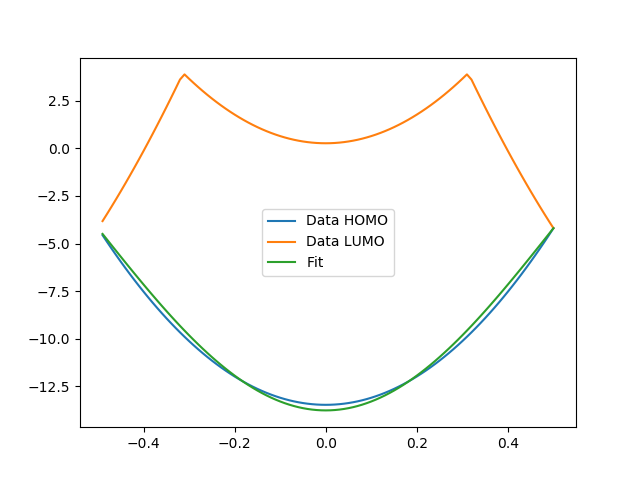
\includegraphics[width = 12cm]{Images/Hydrogen/hydrogen_bandstructure}
	\caption{$E(k)$}
	\label{image_hydrogen_bandstructure}
\end{figure}

In the next step the band structures for the periodically charged hydrogen atoms will be calculated (see \cref{image_hydrogen_charged_bands}). As expected from the symmetry the band structures do not depend on the direction (sign) of the charge displacement. It can also be seen, that the influence of charging is bigger for $k$-points closer to the edge of the Brillouin zone and the bands become shifted to lower energies. Both is in good agreement with the predictions of the Hamiltonian.

\begin{figure}
	\centering
	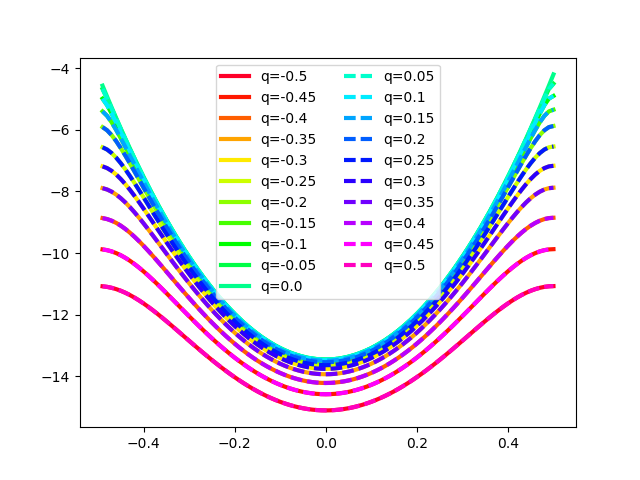
\includegraphics[width = 12cm]{Images/Hydrogen/hydrogen_charged_bands}
	\caption{$E(k, q)$}
	\label{image_hydrogen_charged_bands}
\end{figure}

In \cref{image_hydrogen_charge_potential} the height of the Gaussian potentials causing the charge displacement as a function of the transferred charge is shown. Again the symmetry is as expected and in the region of $-0.2 \le q \le 0.2$ the dependency is approximately linear.

\begin{figure}
	\centering
	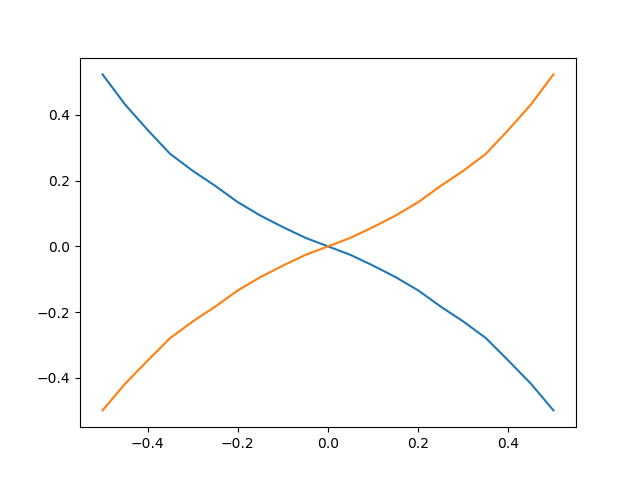
\includegraphics[width = 12cm]{Images/Hydrogen/hydrogen_charge_potential}
	\caption{$V(q)$}
	\label{image_hydrogen_charge_potential}
\end{figure}

For the energy of the 

\begin{figure}
	\centering
	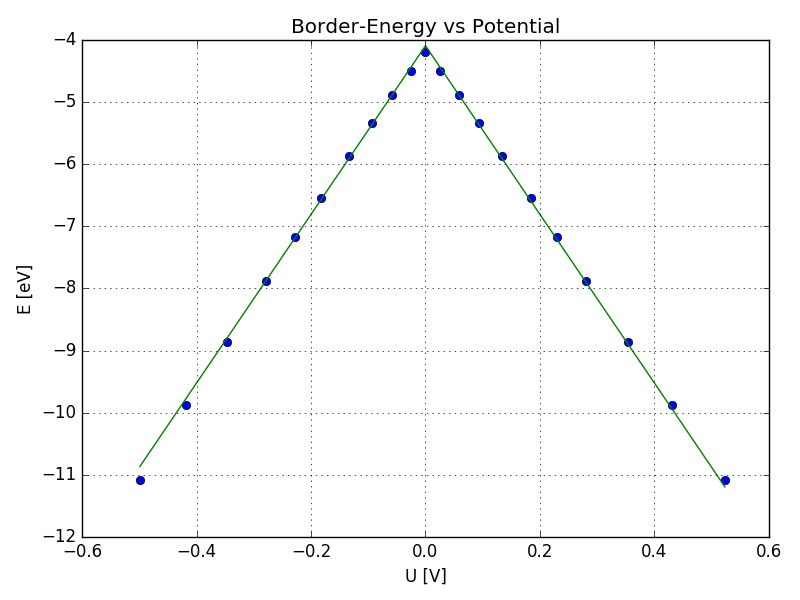
\includegraphics[width = 12cm]{Images/Hydrogen/hydrogen_border_energy}
	\caption{$E(q)$}
	\label{image_hydrogen_charge_potential}
\end{figure}
